\chapter{Introduction} 
\label{Chapter 1} 
\lhead{Chapter 1. \emph{Introduction}} 



\section{Background}
\subsection{API Server}
\subsubsection{What is an API server?}
An Application Programming Interface or API is a software intermediary that allows for the communication between 2 applications or endpoints. APIs can be categorized into 4, namely 
\begin{description}
\item[$\bullet$] Public APIs
\item[$\bullet$] Internal APIs
\item[$\bullet$] Partner APIs
\item[$\bullet$] Composite APIs
\end{description}


An API server is an application that enables another application to exchange information with the server using the API through the internet.
\subsubsection{How does an API sever work?}
Almost always an API sever is up and running either in an on - premise system or in the cloud, listening for requests. When it receives a request it performs the corresponding action, whether it is fetching data, modifying data or even deleting data and sends back a response according to the request.
\subsection{Runner}
\subsubsection{What is a Runner?}
A runner is a virtual machine with a set of custom software, hosted either by a service provider or on our own machines to help execute various custom work-flows which we desire. The main use of a runner is that it can be tied to a pipeline, so that work-flows can be automatically triggered without manual interference. GitHub provides runner software which can be loaded on a machine, and can be used to run GitHub actions, custom work-flows and custom jobs. 
\subsubsection{How does a Runner work?}
A runner is typically tied with a pipeline, and requests are given to the runner based on the current action to be performed within the pipeline. The linking of the pipeline with a runner is usually performed using access tokens.

\section{Motivation}
\subsection{Why use an API server?}
An internal API can be always use to abstract away unnecessary details. Within a large enterprise, it is important that an organization only gets the minimum information needed to function properly. Using APIs can help us achieve this.
Public APIs such as Google maps API, Covid API etc have helped us gain access useful information.
\subsection{Why use a Runner?}
A runner is important to run tasks without human intervention. Automation is a vital part in improving the reliability and efficiency in the computing world and runners can help achieve that.
\section{Objectives of the work}
\subsection{GitHub API Server}
Create an internal API server that can serve requests from ServiceNow(An internal ticketing application), with capabilites to retrieve information from the Github database, change information in the Github database and also delete information in the Github database for the AMD enterprise account and send back appropriate responses back to ServiceNow.
\subsection{GitHub runner}
Create a self - hosted Github runner with capabilities as requested by various other internal organizations and host it in the cloud, which can help them run custom work-flows, jobs and also Github actions.

\begin{figure}[H]
\centering
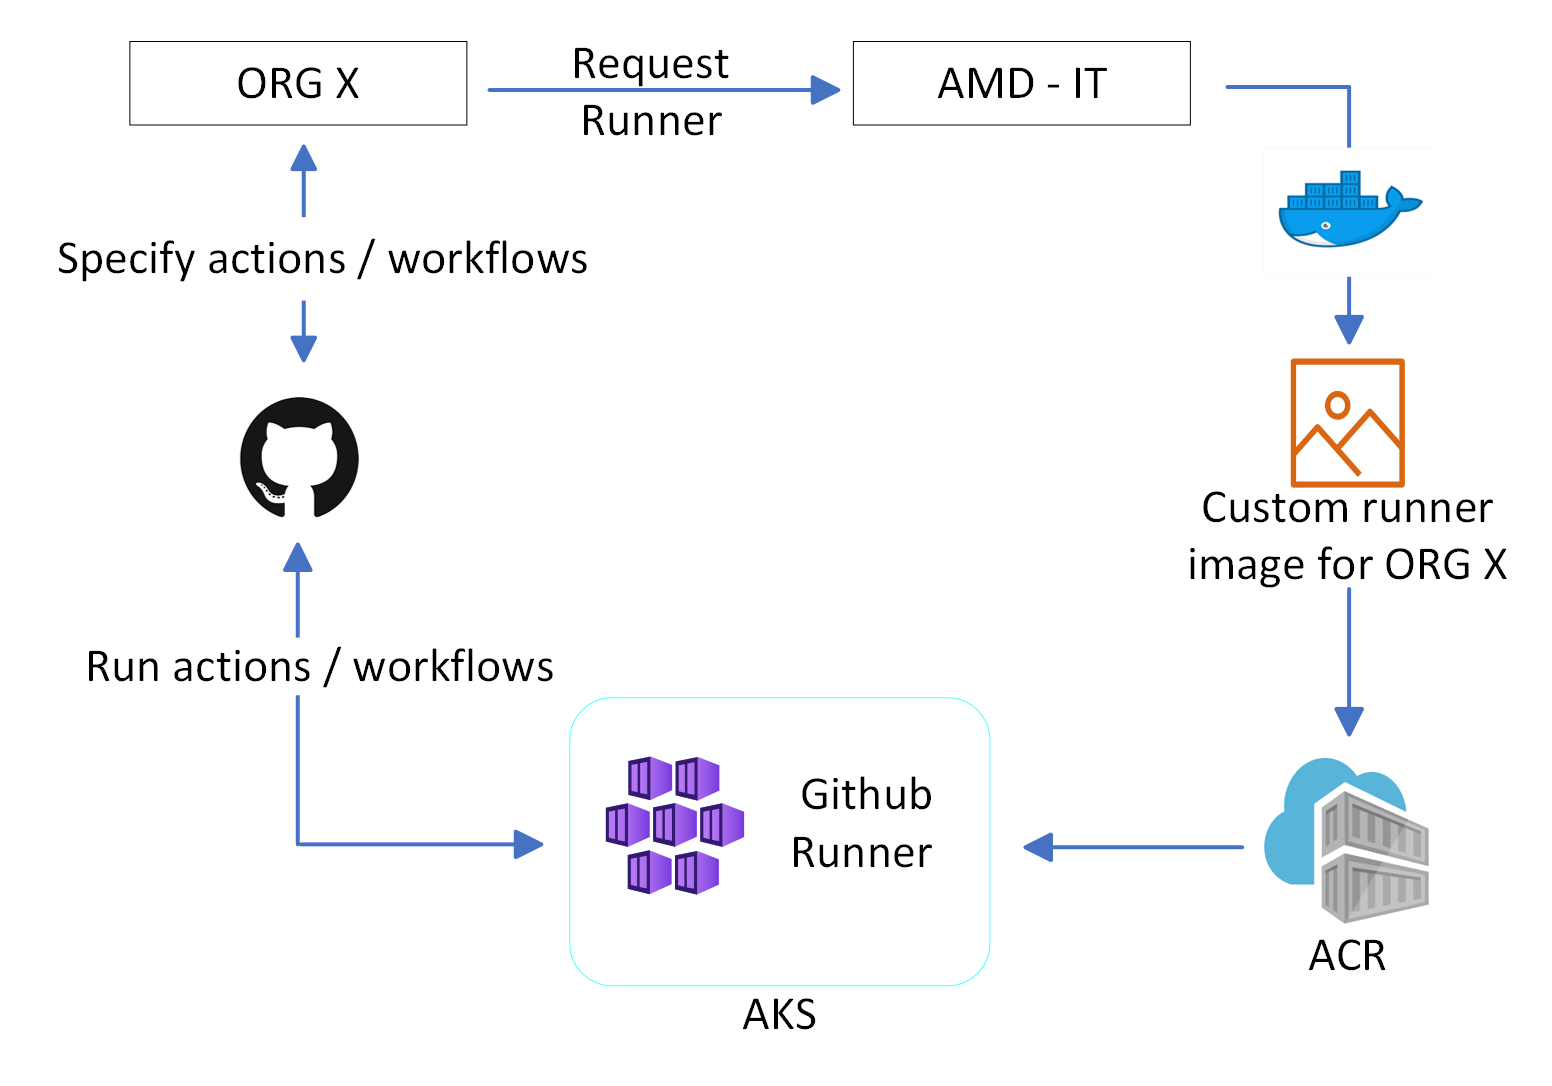
\includegraphics[width = .7\linewidth]{Images/RUNNEROVERVIEW}
\caption{Github Runner Overview}
\label{Github Runner Overview}
\end{figure}
